\documentclass[10pt]{extarticle}
\usepackage{amsmath}
\usepackage{amsfonts}
\usepackage{amssymb}
\usepackage{extsizes}
\usepackage{float}
\usepackage{graphicx}
\usepackage[margin = 1in]{geometry}
\usepackage{hyperref}

\newcommand{\E}{\mathbb{E}}
\newcommand{\Var}{\mathrm{Var}}
\renewcommand{\vec}[1]{\mathbf{#1}}
\newcommand{\Cov}{\mathrm{Cov}}
\begin{document}
	
\title{Bayesian Data Analysis Assignment 1}
\author{Benjamin Cox, S1621312}
\date{\vspace{-5ex}}
\maketitle

\section*{Question 1}

\subsection*{a)}
Our probability vector is $\theta = (\theta_1, \dots, \theta_6)$ and our outcome vector is $c = (c_1, \dots, c_6).$ We are drawing from a multinomial distribution (in the same way that 10 Bern(p) trials are the same as 1 Bin(10,p) trial distributionally), ie $$c \sim \mathrm{Multinomial}(120, \theta).$$ Therefore the likelihood of $\theta$ given $c$ with $n$ trials is the following: $$L(\theta|c) = \frac{n!}{c_1!c_2!\cdots c_6!}\theta_1^{c_1}\cdots\theta_6^{c_6}.$$ A suitable conjugate prior for this would be the Dirichlet distribution (K is the number of possible outcomes, in our case 6), $$f(x| \alpha, K) = \frac{\Gamma(\sum_{i=1}^{K}\alpha_i)}{\prod_{i=1}^{k}\Gamma(\alpha_i)}\prod_{i=1}^{K}x_i^{\alpha_i-1}.$$
The Jeffrey's prior for the multinomial corresponds to a Dirichlet distribution with $$\alpha_i = 1/2\  \forall i\in \{1,\dots,K\}.$$

\subsection*{b)}
Our posterior distribution for $\theta$ is 
\begin{align*}
p(\theta|c) &\propto \left(\frac{\Gamma(3)}{\Gamma(0.5)^6}\theta_1^{-1/2}\cdots\theta_6^{-1/2}\right)\left(\frac{n!}{c_1!c_2!\cdots c_6!}\theta_1^{c_1}\cdots\theta_6^{c_6}\right)\\
&= \mathrm{Dirichlet}\left(\alpha = c+0.5, K = 6\right).
\end{align*}
The expected value of the Dirichlet Distribution is given by $\E\left[X_i\right] = \frac{\alpha_i}{\sum\alpha_i}$, so in our case $$\E\left[\theta_i|c\right] = \frac{c_i+\frac{1}{2}}{\sum c_i + 3}.$$

This corresponds to values of 
\begin{table}[H]
	\centering
	\begin{tabular}{rrrrrrr}
		\hline
		$\E\left[\theta_1\right]$ & $\E\left[\theta_2\right]$ & $\E\left[\theta_3\right]$ & $\E\left[\theta_4\right]$ & $\E\left[\theta_5\right]$ & $\E\left[\theta_6\right]$ \\ 
		\hline
		0.142 & 0.199 & 0.183 & 0.142 & 0.199 & 0.134 \\ 
		\hline
	\end{tabular}
\end{table}

We are going to compute symmetric 95\% credible intervals for each $\theta_i$, hence we must marginalise them. We could (theoretically) calculate a 95\% credible region in the 6 dimensional parameter space, but this would get extremely complicated really quickly, and would also be hard to interpret. 

Fortunately the marginal distributions of the Dirichlet are a lot easier, as they are beta distributions. Write $\alpha_0 = \sum\alpha_k,$ then we have 
$$\theta_i \sim \mathrm{Beta}\left(\alpha_i, \alpha_0 - \alpha_i\right).$$ We can substitute in our expressions for $\alpha_i$ to obtain $$\theta_i \sim \mathrm{Beta}\left(c_i + 1/2, c_0 - c_i + 2.5\right).$$ Using this result we obtain the following 95\% credible intervals:


\begin{table}[H]
	\centering
	\begin{tabular}{r|rr}
		\hline
		$\theta$ & Lower & Upper\\
		\hline
		$\theta_1$ & 0.08657456 &0.20897331\\
		$\theta_2$ &0.1337529 &0.2738778\\
		$\theta_3$ &0.1200040 &0.2556043\\
		$\theta_4$ &0.08657456 &0.20897331\\
		$\theta_5$ &0.1337529 &0.2738778\\
		$\theta_6$ &0.08007849 &0.19945622\\
	\end{tabular}
\end{table}

\subsection*{c)}
We are going to test the null hypothesis of a fair die. For the multinomial distribution there is no easy quantile function, so we are going to use the likelihood-ratio test and Pearson's $\chi^2$ test. These approach the true $p$-value from below and above respectively, so doing both should give us a very good idea.

Computing the $p$-value using the likelihood-ratio test we get $p_{lr} = 0.377$. Computing the $p$-value using Pearson's $\chi^2$ test we obtain $p_{\chi^2} = 0.377$. Thus we can be fairly sure that this is very close to the true $p$-value. Therefore we do not reject the null hypothesis that the die is fair.

\subsection*{d)}
The posterior predictive distribution is the `Dirichlet-Multinomial' distribution. The pmf for this is given by 
\[
f(x|n, \alpha) = \frac{n!\Gamma(\sum\alpha_i)}{\Gamma(n+\sum\alpha_i)}\prod_{k=1}^{K}\frac{\Gamma(x_k+\alpha_k)}{(x_k!)\Gamma(\alpha_k)}
\]
for $n$ the number of trials and $alpha_1, \dots, \alpha_k > 0.$ 

Taken as our posterior predictive under the Jeffrey's prior we have $$c_{\text{new}}\sim \mathrm{DirMNom(60, c + 1/2)}.$$
We can simulate from this. We draw 10,000 times from this distribution and find that with probability 0.737 we have more 5s than 6s in our next 60 trials.

\subsection*{e)}
We incorporate these into our likelihood, denoting the new count vector as $d$. Our new posterior is $$\theta \sim \mathrm{Dirichlet}(c+d+1/2, 6).$$ Our new posterior means are 
\begin{table}[H]
	\centering
	\begin{tabular}{rrrrrrr}
		\hline
		$\E\left[\theta_1\right]$ & $\E\left[\theta_2\right]$ & $\E\left[\theta_3\right]$ & $\E\left[\theta_4\right]$ & $\E\left[\theta_5\right]$ & $\E\left[\theta_6\right]$ \\ 
		\hline
		0.163 &0.183 &0.216 &0.138 &0.167 &0.138 \\ 
		\hline
	\end{tabular}
\end{table}
with 95\% marginal credible intervals given by 
\begin{table}[H]
	\centering
	\begin{tabular}{r|rr}
		\hline
		$\theta$ & Lower & Upper\\
		\hline
		$\theta_1$ &0.1189814 &0.2113785\\
		$\theta_2$ &0.1371556 &0.2340370\\
		$\theta_3$ &0.1667039 &0.2698204\\
		$\theta_4$ &0.0975285 &0.1838316\\
		$\theta_5$ &0.1225962 &0.2159303\\
		$\theta_6$ &0.0939960 &0.1791973\\
	\end{tabular}
\end{table}
The credible intervals have narrowed, as expected for more observations. It is of note that the new credible interval for $\theta_3$ (barely) does not contain the value required for a `fair' dice. This is evidence that the dice is not fair. 

\section*{Question 2}

\subsection*{a)}

We have two equally credible opinions on the distribution of $1/\lambda$. We have one stating that it lies mostly between 5 and 10, and another that states that it lies between 0 and 25. We are going to use the Gamma distribution as our prior for $\lambda$. 

We are going to calculate parameters for this such that the corresponding inverse gamma distributions has mean of the midpoint and standard deviation of 1/4 the range. 

Calculating these parameters we obtain 
\[
\alpha_1 = 38, \beta_1 = 277.5, \qquad \alpha_2 = 6, \beta_2 = 62.5,
\]
with the indices corresponding to the originating expert.

This means that our mixture prior is of the form 
\[
\lambda \sim 0.5\cdot\Gamma(38, 277.5) + 0.5\cdot\Gamma(6, 62.5)
\]

\subsection*{b)}

We have 100 points of data with a mean of 9.877 minutes. We calculate our posterior. The gamma distribution is a conjugate prior to the exponential distribution, so it is quite simple to calculate our new parameters. 

We calculate 
\[
\alpha_1^{post} = 138, \beta_1^{post} = 1265.2, \qquad \alpha_2^{post} = 106, \beta_2^{post} = 1050.2
\] using the formulae $\alpha^{post} = \alpha + n, \beta^{post} = \beta + \sum_i x_i = \beta + n\bar{x}.$ To calculate the posterior mixing proportion $Q$ we use \[Q = \frac{q\frac{\beta_1^{\alpha_1}}{\Gamma(\alpha_1)}\frac{\Gamma(\alpha_1^{post})}{\beta_1^{post \ \alpha_1^{post}}}}{q\frac{\beta_1^{\alpha_1}}{\Gamma(\alpha_1)}\frac{\Gamma(\alpha_1^{post})}{\beta_1^{post \ \alpha_1^{post}}} + (1-q)\frac{\beta_2^{\alpha_2}}{\Gamma(\alpha_2)}\frac{\Gamma(\alpha_2^{post})}{\beta_2^{post \ \alpha_2^{post}}}}.\]
This quantity involves extremely large numbers, so we work on the log scale and exponentiate at the end. 

Overall we obtain a posterior of the form
\[
p(\lambda|x) = 0.40455 \cdot \Gamma(138, 1265.2) + 0.59545 \cdot \Gamma(106, 1050.2). 
\]

Of course the posterior for $1/\lambda$ is analogous, with inverse gamma rather than gamma.

We calculate a posterior 95\% credible interval for $1/\lambda$ as $(8.00, 11.84)$, and a mean for $1/\lambda$ of 9.69.

To calculate the posterior probability of waiting for more than 20 minutes we need the posterior predictive distribution. We find that $$\Pr[x>20] = 0.127.$$ We note that the posterior distribution is a gamma mixture whereas the posterior predictive distribution is a generalised Pareto distribution. The pdf is given by 

\[
p(t_*|t) = 0.40455 \ f_l(\beta_1^{post}, \alpha_1^{post}) + 0.59545 \ f_l(\beta_2^{post}, \alpha_2^{post}),
\]

where 
\[
f_l(x|a,b) = \frac{a}{b}\left(1+\frac{x}{b}\right)^{-(a-1)}.
\]
This family of distributions is often used in survival analysis to model survival times, so it is natural that it could turn up here.

\subsection*{c)}
\begin{figure}[H]
	\centering
	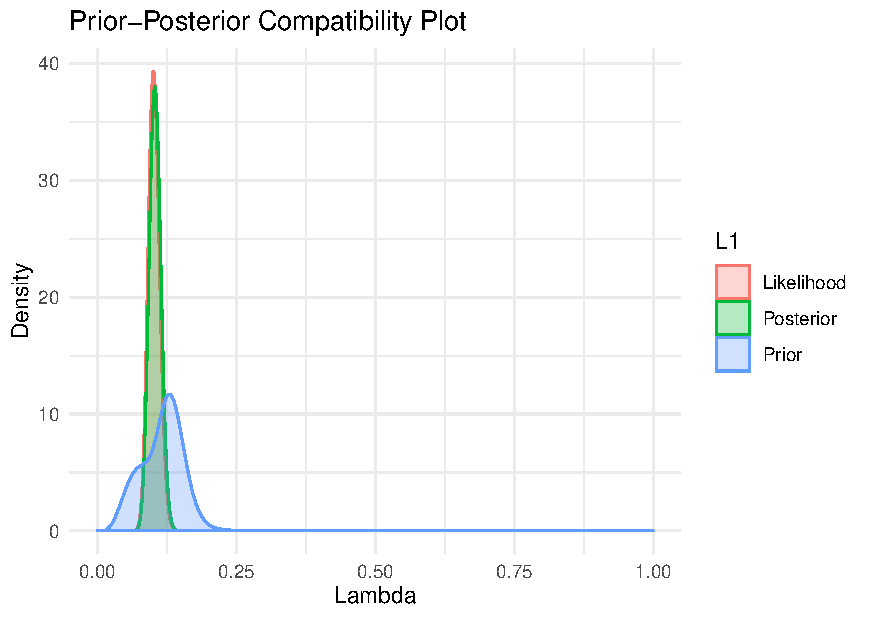
\includegraphics[width = 0.5\textwidth]{../plpgoodnessplot}
	\caption{Prior-Likelihood-Posterior Plot}
	\label{fig:pgof}
\end{figure}

As seen in Figure (\ref{fig:pgof}) the posterior is highly influenced by the likelihood and not so much by the prior. The prior is compatible with the data as an initial estimate, and and served it's purpose well as the posterior has converged (mostly) onto the likelihood.

The prior is compatible as there is no conflict between the data and the posterior.

\subsection*{d)}
\begin{figure}[H]
	\centering
	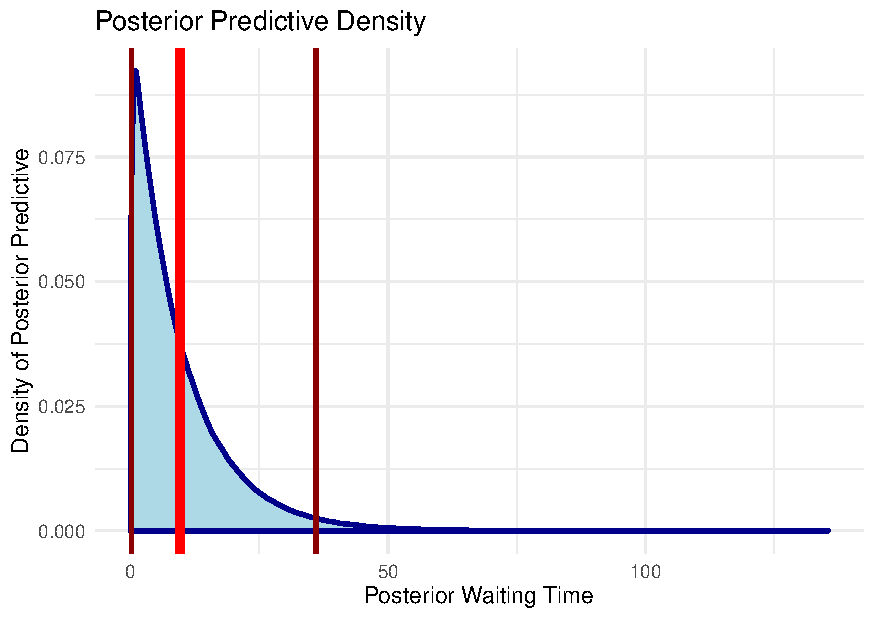
\includegraphics[width = 0.5\textwidth]{../postpreddens}
	\caption{Posterior Predictive Density Plot, bright red line indicates mean, darker red lines indicate 95\% CI.}
	\label{fig:postpreddens}
\end{figure}

We plot our posterior predictive density. We obtain a mean of $9.69$ with symmetric 95\% credible interval given by $(0.24, \  36)$. This is very much in line with what we expect from the likelihood, indicating good fit. 

\subsection*{e)}
We are now to take the Lindley distribution as our likelihood. This distribution has pdf of
\[
f(t|\lambda) = \frac{\lambda^2}{\lambda+1}(1+t)e^{-\lambda t} \implies \ln(f(t|\lambda)) = 2\ln(\lambda) - \ln(\lambda + 1) + \ln(1+t) - \lambda t.
\]
The log pdf is important for implementing into our MC algorithm.  

Given our data we have likelihood of the form 
\[
L(\lambda|\underline{t}) = \left(\frac{\lambda^2}{\lambda+1}\right)^n\exp\left(-\lambda\sum_{i=1}^{n}t_i\right)\prod_{i=1}^{n}(1+t_i),
\]

hence we have a posterior of the form
\begin{align*}
p(\lambda|\underline{t}) &\propto \left(\Gamma(38, 277.5) + \Gamma(6, 62.5)\right)\left(\frac{\lambda^2}{\lambda+1}\right)^n\exp\left(-\lambda\sum_{i=1}^{n}t_i\right)\prod_{i=1}^{n}(1+t_i)\\
&\propto \left(\frac{277.5^{38}}{\Gamma(38)}\lambda^{37}e^{-277.5\cdot \lambda} + \frac{62.5^6}{\Gamma(6)}\lambda^{5}e^{-62.5\cdot \lambda}\right)\left(\frac{\lambda^2}{\lambda+1}\right)^n\exp\left(-\lambda\sum_{i=1}^{n}t_i\right)\prod_{i=1}^{n}(1+t_i)
\end{align*}

We calculate our posterior. We obtain an expected waiting time of $10.4$ minutes, an increase from our previous.

We also plot the new posterior predictive. 

\begin{figure}[H]
	\centering
	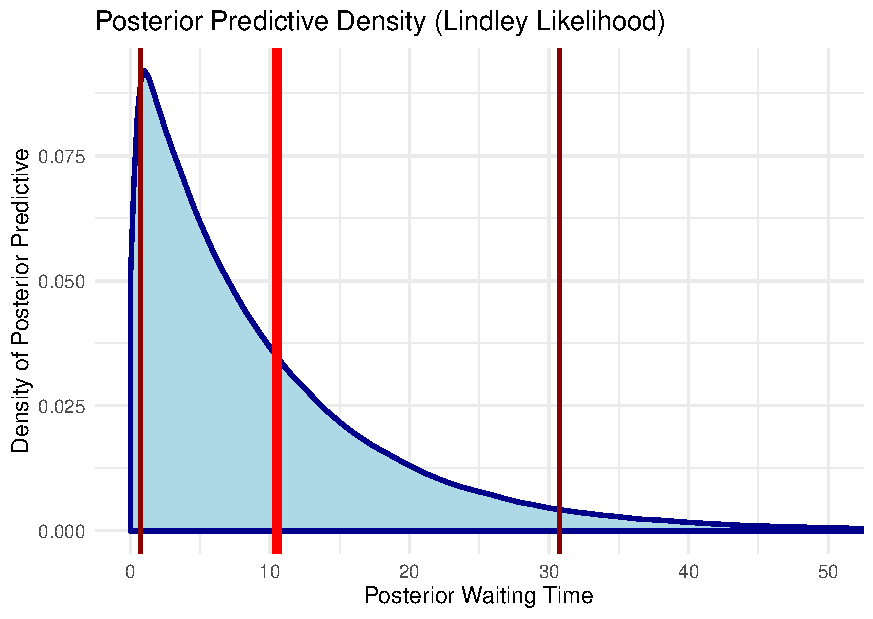
\includegraphics[width = 0.5\textwidth]{../ppredlinddens}
	\caption{Posterior Predictive Density Plot for Lindley Likelihood, bright red line indicates mean, darker red lines indicate 95\% CI.}
	\label{fig:postpredlinddens}
\end{figure}

Notice that the credible interval for the posterior predictive derived from the Lindley likelihood are a lot tighter. 

\subsection*{f)}
\begin{figure}[H]
	\centering
	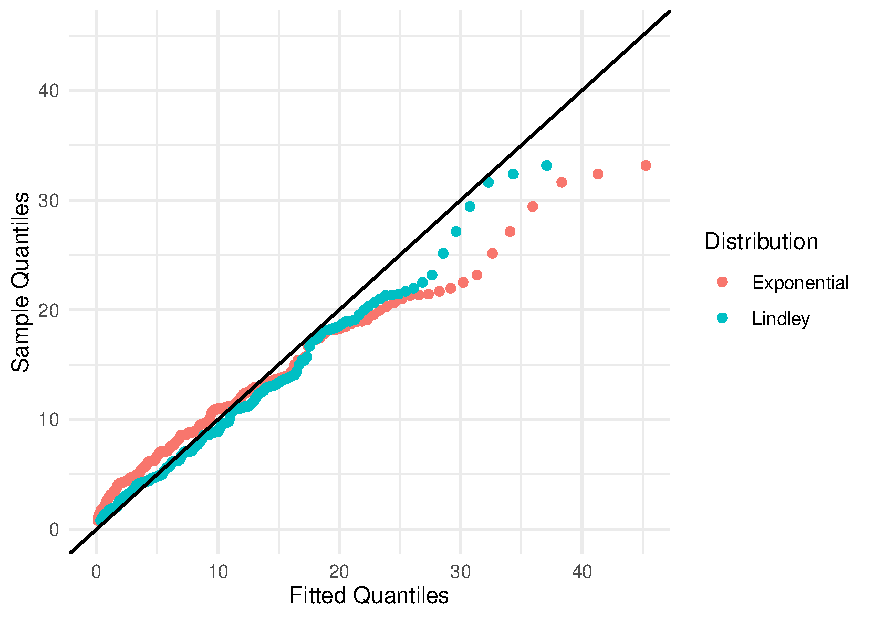
\includegraphics[width = 0.5\textwidth]{../qqplotlindexp}
	\caption{Q-Q plot of sample quantiles against posterior predictive quantiles}
	\label{fig:qqplots}
\end{figure}
We see that the Lindley distribution fits the data much better than the exponential distribution. We perform Kolmogorov-Smirnoff tests comparing our posterior predictives and the data. For the Lindley likelihood we obtain a distance of 0.0685 with $p$-value of 0.736. For the exponential likelihood we obtain a distance of 0.1797 with corresponding $p$-value of 0.003. 

This is extremely good evidence that the Lindley distribution is a better fit for the data than the Exponential distribution. 

\section*{Question 3}
\subsection*{a)} 

In order to make our results directly comparable we are going to mean centre the data before we fit the initial linear model. This should only affect the intercept term. 

\begin{table}[ht]
	\centering
	\begin{tabular}{rrrrr}
		\hline
		& Estimate & Std. Error & t value & Pr($>$$|$t$|$) \\ 
		\hline
		(Intercept) & 0.2439 & 0.0643 & 3.79 & 0.0002 \\ 
		SexI & -0.8249 & 0.1024 & -8.06 & 0.0000 \\ 
		SexM & 0.0577 & 0.0833 & 0.69 & 0.4887 \\ 
		Length & -0.4583 & 1.8091 & -0.25 & 0.8000 \\ 
		Diameter & 11.0751 & 2.2273 & 4.97 & 0.0000 \\ 
		Height & 10.7615 & 1.5362 & 7.01 & 0.0000 \\ 
		Whole.weight & 8.9754 & 0.7254 & 12.37 & 0.0000 \\ 
		Shucked.weight & -19.7869 & 0.8174 & -24.21 & 0.0000 \\ 
		Viscera.weight & -10.5818 & 1.2937 & -8.18 & 0.0000 \\ 
		Shell.weight & 8.7418 & 1.1247 & 7.77 & 0.0000 \\ 
		\hline
	\end{tabular}
\end{table}

This points to length and Male-Female difference not having a significant effect on age. Length is likely due to high correlation with height (Pearson correlation of 0.828) and diameter (Pearson correlation of 0.987). Most of the variables have extremely high correlation, so this is going to require a long MCMC run.

\begin{figure}[H]
	\centering
	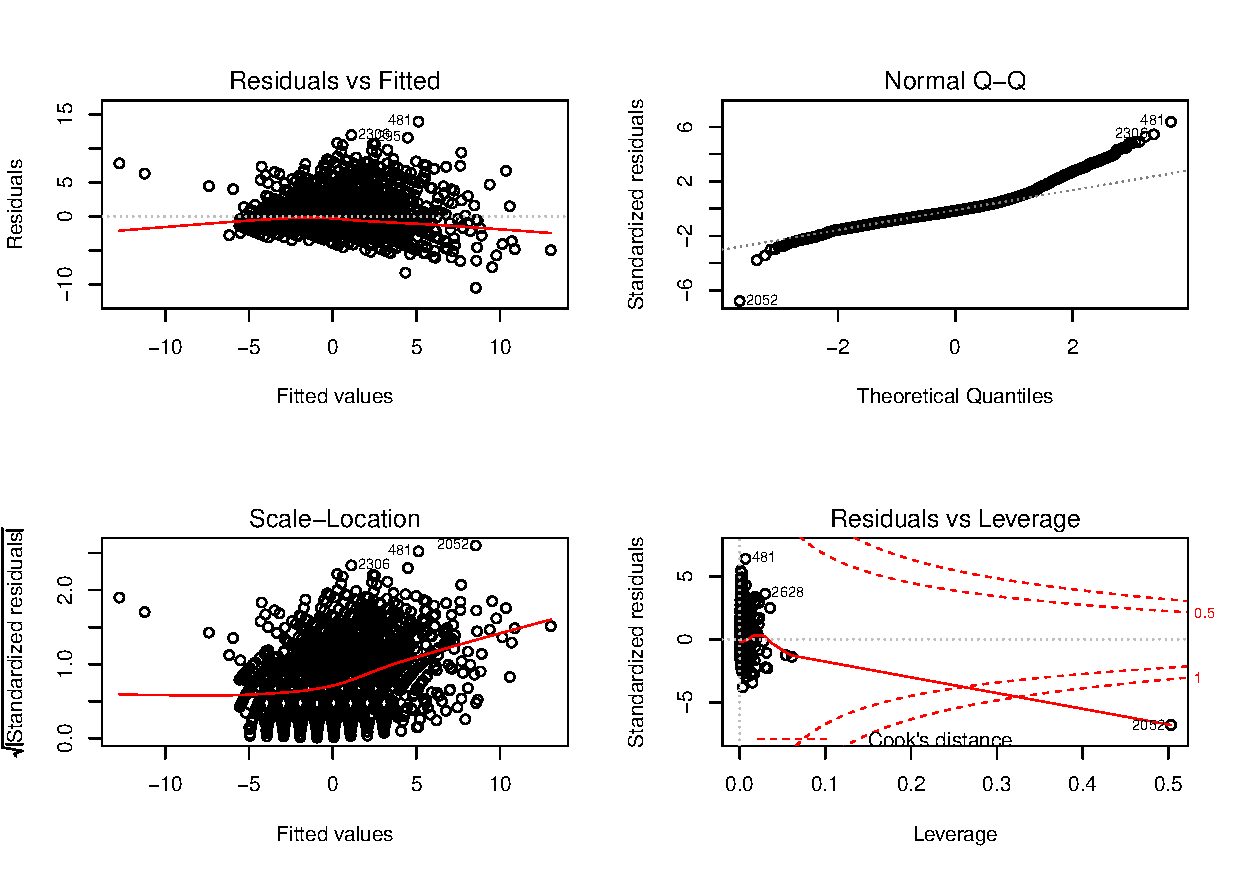
\includegraphics[width = 0.5\textwidth]{../flmdiag}
	\caption{Diagnostic plots for the standard linear model}
	\label{fig:lmplots}
\end{figure}

Looking at diagnostic plots we see a large number of extreme observations with high leverage. Therefore it makes sense to perform a robust regression using $t$ distributed errors.  
\subsection*{b)}

We are going to fit a Bayesian linear model of the form 
\begin{align*}
y &\sim t_{\nu+1}(X\beta, \sigma),\\
\beta_i & \sim \mathrm{Normal}(0, 10^4),\\
\sigma &\sim \Gamma^{-1}(0.1, 0.1),\\
\nu &\sim \mathrm{Exponential}(0.034),
\end{align*}
where $X$ is the $n \times p$ centred design matrix, $\beta$ is the $p$ vector of regression coefficients, and the $t$ distribution is understood to be shifted and scaled such that $\frac{y-X\beta}{\sigma}$ has a classic $t$ distribution with $\nu + 1$ degrees of freedom.

\subsection*{c)}

Fitting the model we obtain the following quantities:
\begin{table}[ht]
	\footnotesize
	\centering
	\begin{tabular}{rrrrrrrrrrr}
		\hline
		& mean & se\_mean & sd & 2.5\% & 25\% & 50\% & 75\% & 97.5\% & n\_eff & Rhat \\ 
		\hline
		beta[1] & -0.22 & 0.00 & 0.06 & -0.33 & -0.25 & -0.22 & -0.18 & -0.11 & 28239.55 & 1.00 \\ 
		beta[2] & -0.67 & 0.00 & 0.08 & -0.83 & -0.73 & -0.67 & -0.61 & -0.51 & 32862.97 & 1.00 \\ 
		beta[3] & 0.12 & 0.00 & 0.07 & -0.02 & 0.07 & 0.12 & 0.17 & 0.26 & 33774.18 & 1.00 \\ 
		beta[4] & 1.88 & 0.01 & 1.51 & -1.13 & 0.86 & 1.89 & 2.90 & 4.82 & 31346.96 & 1.00 \\ 
		beta[5] & 7.28 & 0.01 & 1.86 & 3.64 & 6.02 & 7.27 & 8.53 & 10.96 & 31154.47 & 1.00 \\ 
		beta[6] & 15.80 & 0.01 & 2.04 & 11.81 & 14.43 & 15.80 & 17.17 & 19.80 & 50288.95 & 1.00 \\ 
		beta[7] & 7.51 & 0.01 & 0.80 & 5.94 & 6.97 & 7.51 & 8.04 & 9.06 & 23090.61 & 1.00 \\ 
		beta[8] & -16.35 & 0.01 & 0.90 & -18.12 & -16.95 & -16.35 & -15.74 & -14.59 & 26678.37 & 1.00 \\ 
		beta[9] & -9.22 & 0.01 & 1.20 & -11.56 & -10.03 & -9.22 & -8.41 & -6.89 & 34525.85 & 1.00 \\ 
		beta[10] & 6.72 & 0.01 & 1.17 & 4.43 & 5.92 & 6.71 & 7.50 & 9.05 & 28005.24 & 1.00 \\ 
		sigma & 1.39 & 0.00 & 0.03 & 1.33 & 1.37 & 1.39 & 1.41 & 1.45 & 35667.27 & 1.00 \\ 
		nu & 1.87 & 0.00 & 0.16 & 1.58 & 1.76 & 1.86 & 1.97 & 2.19 & 35705.46 & 1.00 \\ 
		y\_new[1] & -0.34 & 0.01 & 2.47 & -4.85 & -1.41 & -0.34 & 0.74 & 4.22 & 56374.07 & 1.00 \\ 
		lp\_\_ & -6470.43 & 0.02 & 2.47 & -6476.21 & -6471.85 & -6470.08 & -6468.65 & -6466.64 & 21223.39 & 1.00 \\ 
		\hline
	\end{tabular}
\caption{Regression Coefficient Table}
\label{tab:regco}
\end{table}

\subsection*{d)}

The model table contains our $\hat{R}$ values, and shows that we have good reason to believe that the chains have converged. 

\begin{figure}[H]
	\centering
	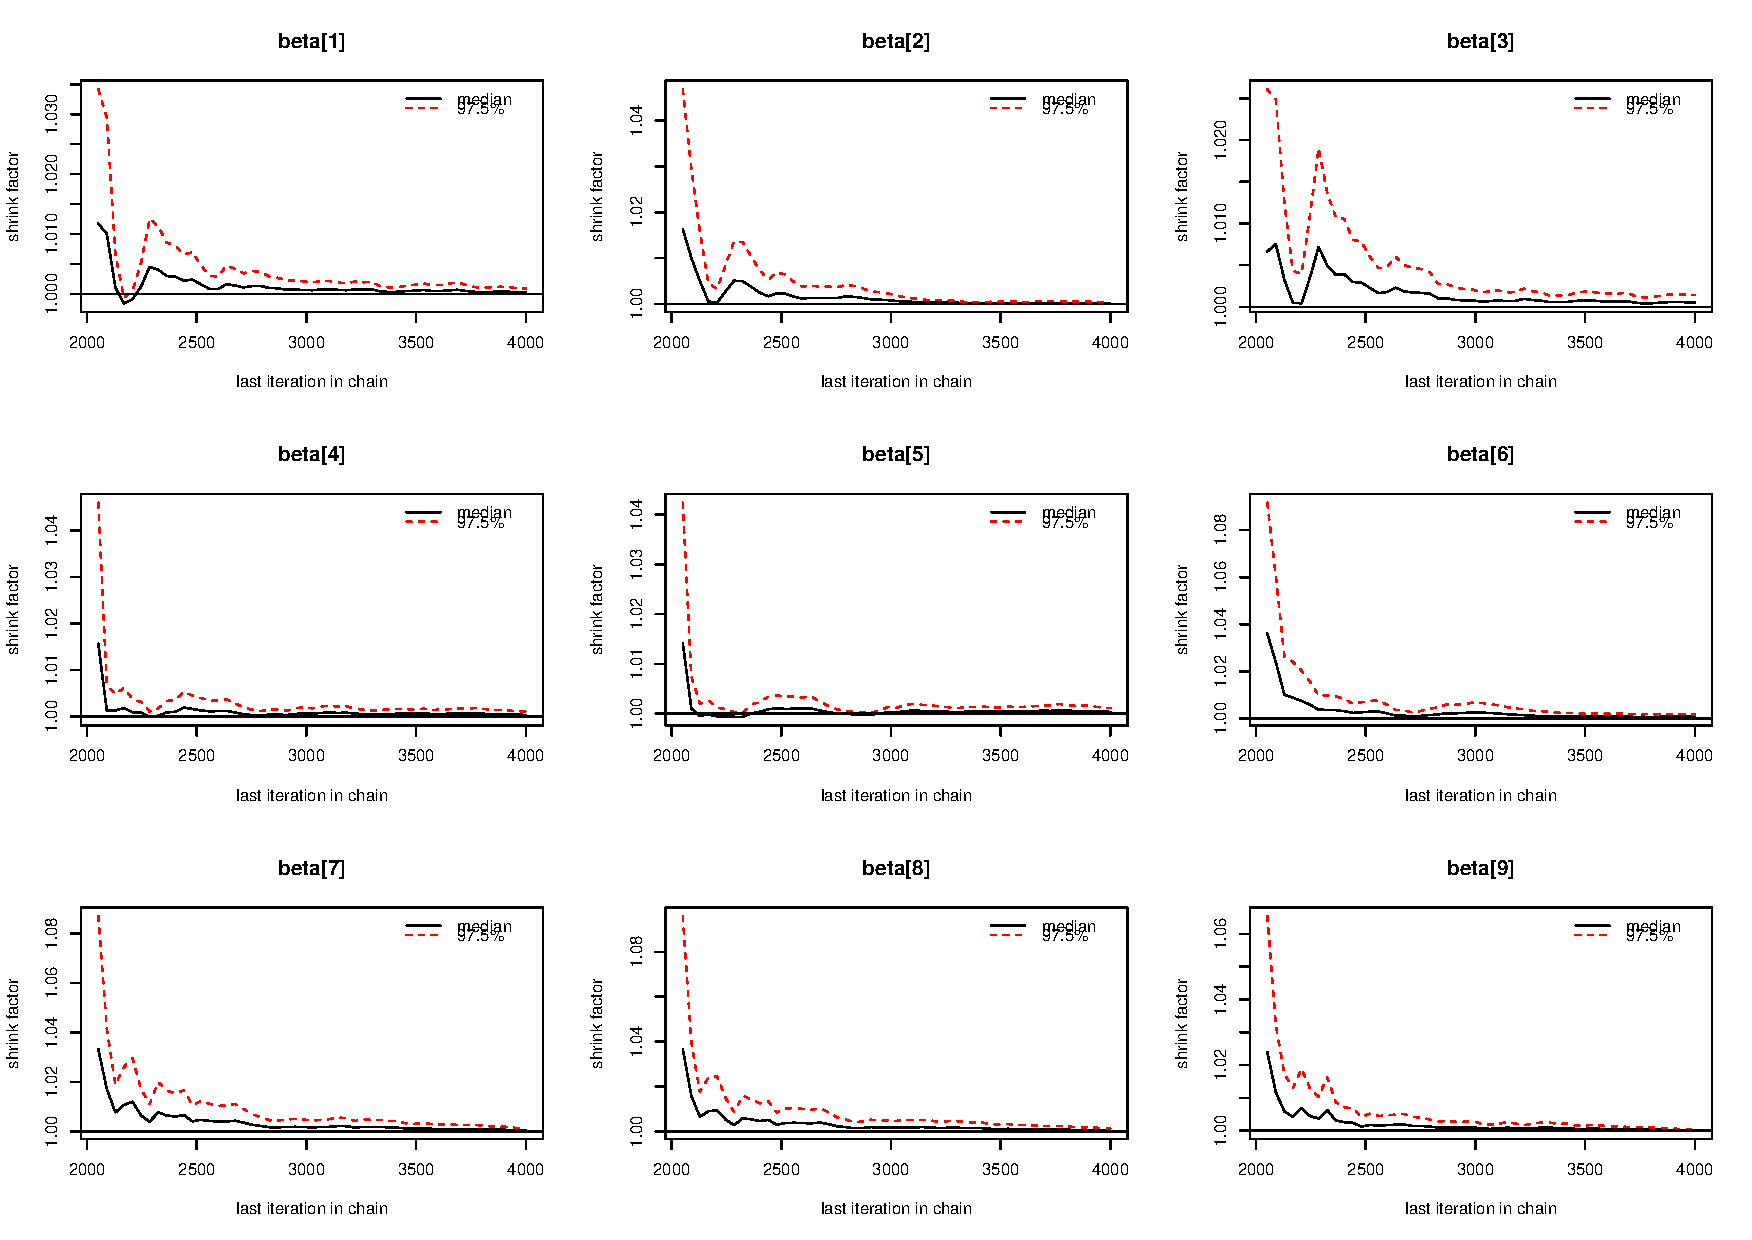
\includegraphics[width = 0.45\textwidth]{../gelman1}
	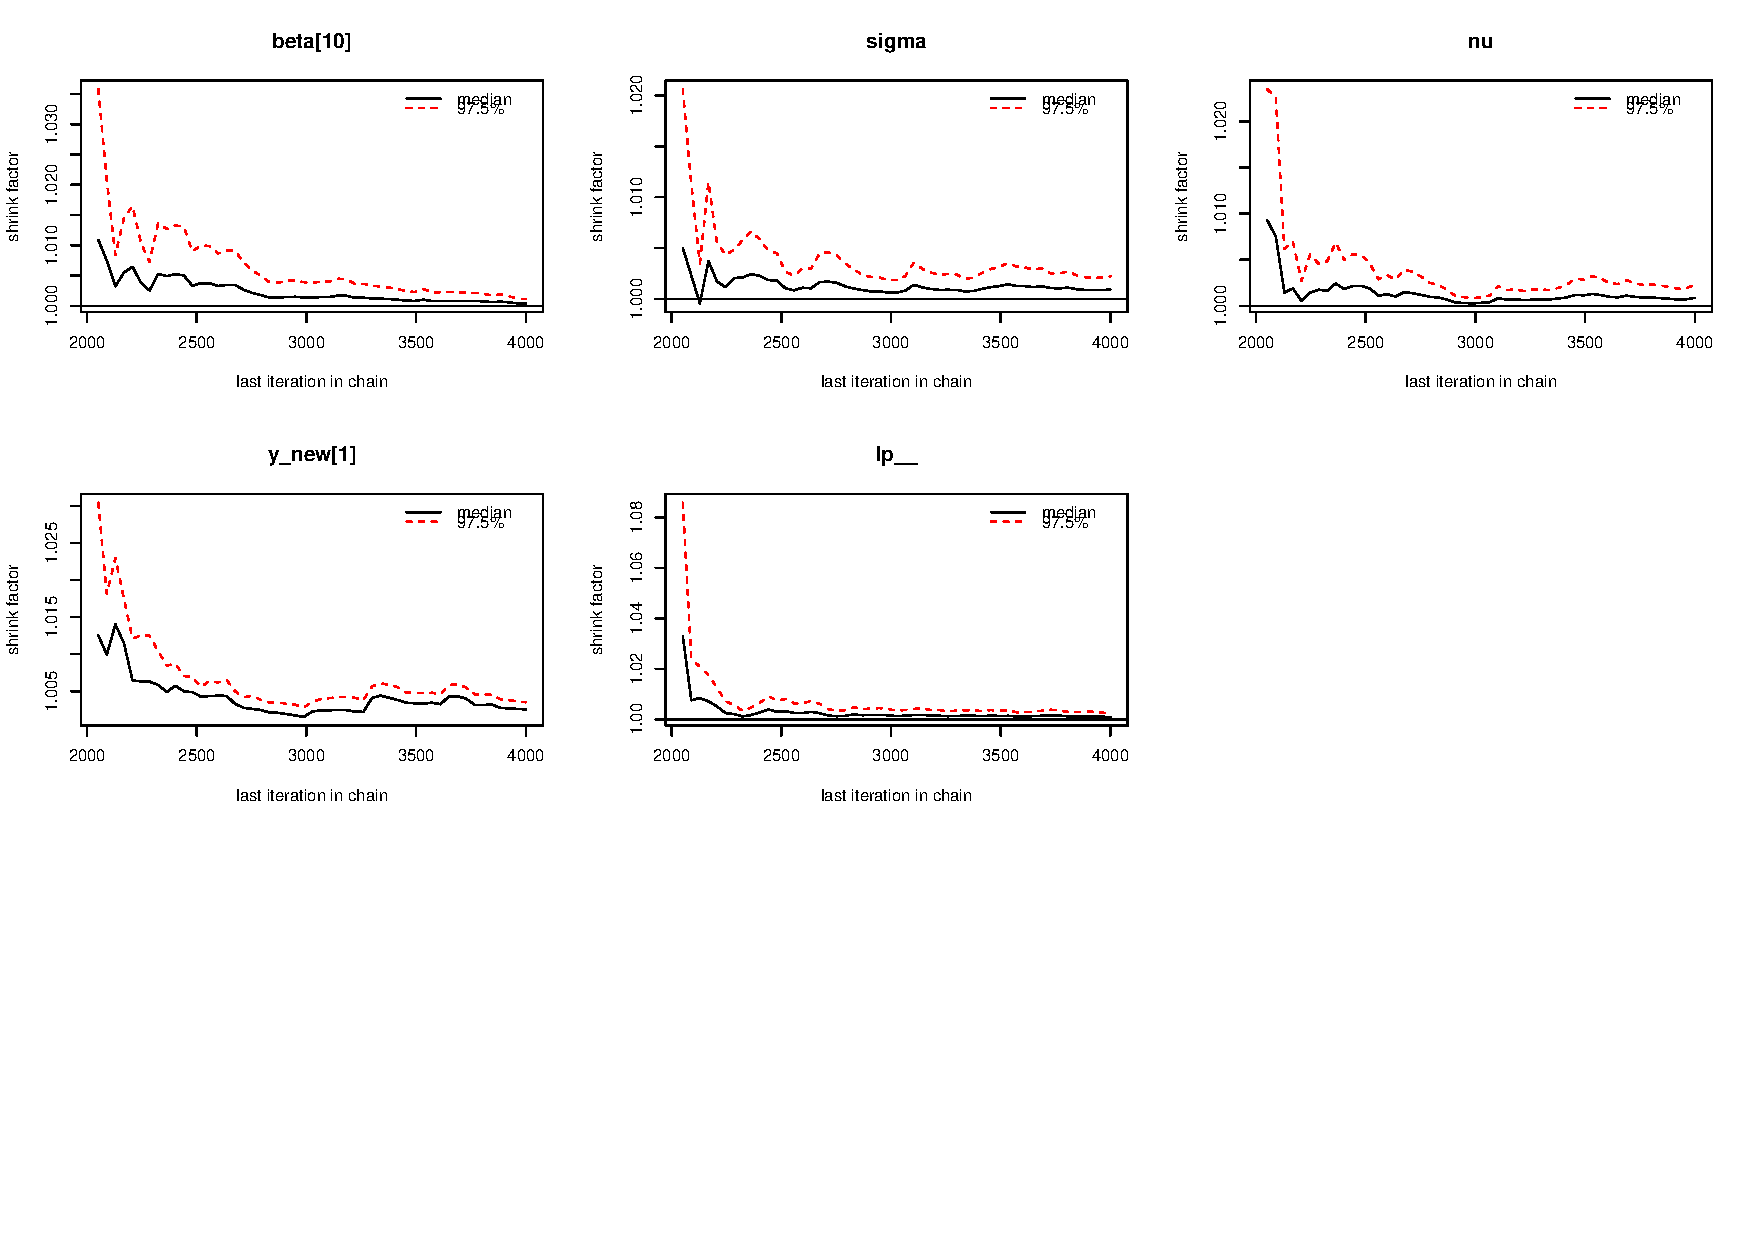
\includegraphics[width = 0.45\textwidth]{../gelman2}
	\caption{Plots of $\hat{R}$ as chains progressed}
	\label{fig:gelmanplots}
\end{figure}

Although Figure \ref{fig:gelmanplots} is a bit small it is clear that after our burn-in $\hat{R}$ was very close to 1, and got closer as we computed more iterations.

\subsection*{e)}

We are going to alter some of the prior hyperparameters in order to test sensitivity. We are going to assume the following model:

\begin{align*}
y &\sim t_\nu(X\beta, \sigma),\\
\beta_i & \sim \mathrm{Normal}(0, 10),\\
\sigma &\sim \Gamma^{-1}(7, 30),\\
\nu &\sim \mathrm{Exponential}(0.034),
\end{align*}
The hyperparameters are quite different, so this should be a good test of prior sensitivity. We are going to run the model for less iterations as we do not intend to use this model for inference, merely for prior sensitivity analysis.

We obtain the following table of results: 

\begin{table}[ht]
	\tiny
	\centering
	\begin{tabular}{rrrrrrrrrrr}
		\hline
		& mean & se\_mean & sd & 2.5\% & 25\% & 50\% & 75\% & 97.5\% & n\_eff & Rhat \\ 
		\hline
		beta[1] & -0.21 & 0.00 & 0.06 & -0.32 & -0.25 & -0.21 & -0.17 & -0.10 & 5572.99 & 1.00 \\ 
		beta[2] & -0.68 & 0.00 & 0.08 & -0.84 & -0.73 & -0.68 & -0.62 & -0.51 & 6239.80 & 1.00 \\ 
		beta[3] & 0.12 & 0.00 & 0.07 & -0.02 & 0.07 & 0.12 & 0.17 & 0.25 & 6566.89 & 1.00 \\ 
		beta[4] & 1.98 & 0.02 & 1.47 & -0.89 & 0.97 & 1.98 & 2.99 & 4.82 & 6567.40 & 1.00 \\ 
		beta[5] & 7.23 & 0.02 & 1.80 & 3.71 & 5.98 & 7.24 & 8.46 & 10.72 & 6482.90 & 1.00 \\ 
		beta[6] & 15.25 & 0.02 & 2.01 & 11.29 & 13.91 & 15.27 & 16.63 & 19.13 & 9565.22 & 1.00 \\ 
		beta[7] & 7.36 & 0.01 & 0.78 & 5.82 & 6.83 & 7.36 & 7.89 & 8.86 & 4357.55 & 1.00 \\ 
		beta[8] & -16.20 & 0.01 & 0.90 & -17.95 & -16.81 & -16.20 & -15.60 & -14.44 & 4957.90 & 1.00 \\ 
		beta[9] & -8.98 & 0.01 & 1.19 & -11.31 & -9.78 & -9.00 & -8.19 & -6.64 & 6498.79 & 1.00 \\ 
		beta[10] & 6.93 & 0.02 & 1.15 & 4.74 & 6.15 & 6.91 & 7.70 & 9.25 & 5590.50 & 1.00 \\ 
		sigma & 1.40 & 0.00 & 0.03 & 1.34 & 1.38 & 1.40 & 1.42 & 1.46 & 6930.44 & 1.00 \\ 
		nu & 1.90 & 0.00 & 0.16 & 1.61 & 1.79 & 1.89 & 2.00 & 2.22 & 7134.90 & 1.00 \\ 
		y\_new[1] & -0.36 & 0.02 & 2.54 & -4.77 & -1.41 & -0.35 & 0.72 & 4.13 & 10775.23 & 1.00 \\ 
		lp\_\_ & -6497.93 & 0.04 & 2.39 & -6503.44 & -6499.35 & -6497.65 & -6496.19 & -6494.16 & 4370.59 & 1.00 \\ 
		\hline
	\end{tabular}
\end{table}

This is nearly identical to the table obtained previously, so we can be confident in our results. All of the differences in means are well within their standard deviations, so overall we are happy.

\subsection*{f)}

\begin{figure}[H]
	\centering
	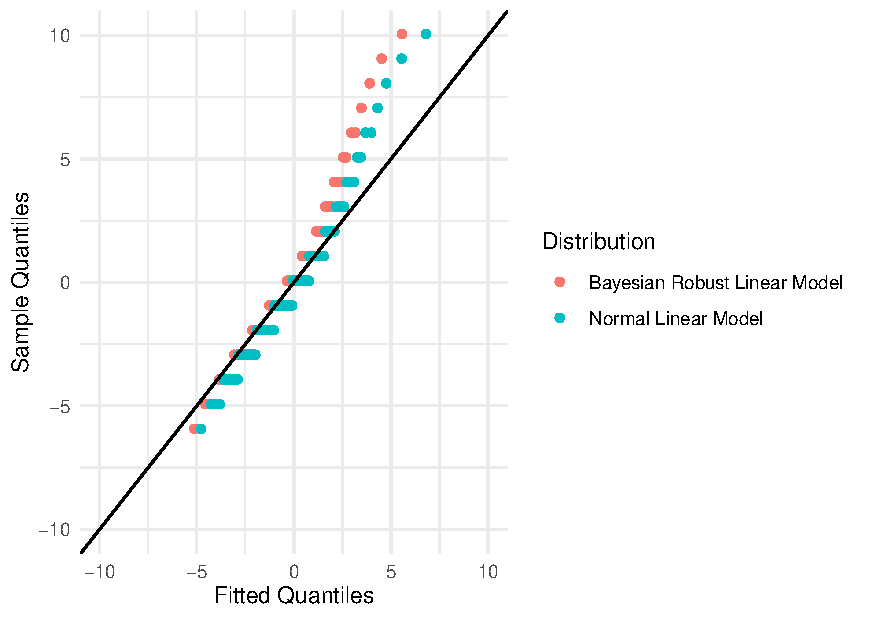
\includegraphics[width = 0.5\textwidth]{../qqplotmodcomp}
	\caption{QQ plots comparing our models}
	\label{fig:qqp}
\end{figure}
Looking at figure \ref{fig:qqp} neither of our models fit the data very well. Performing KS tests we find a distance of 0.11827 between our predictions from the Robust Bayesian and the true data, compared with a distance of 0.15466 for the normal linear and the true data. We note that the true data is rather skewed with estimated skewness 1.11. This has not been compensated for in the model. This means that there are more old abalones than predicted by the models. This is likely due to their characteristics not changing that much after they age enough. This is shown by the deviation of the upper quantiles of the predictions from the sample quantiles.

\subsection*{g)}

95\% credible intervals are given in Table \ref{tab:regco}. We see that the credible intervals for $\beta_3$ and  $\beta_4$ contain 0. These are the coefficients linked to `isMale' and Length respectively. This observation is identical to that of the normal linear model. 

\subsection*{h)}

The 95\% credible interval for the age relating to the  new data is given in the Table \ref{tab:regco} as $(-4.85, 4.22)$ with mean of $-0.34$. We plot the density of the posterior predictive and obtain the following:

\begin{figure}[H]
	\centering
	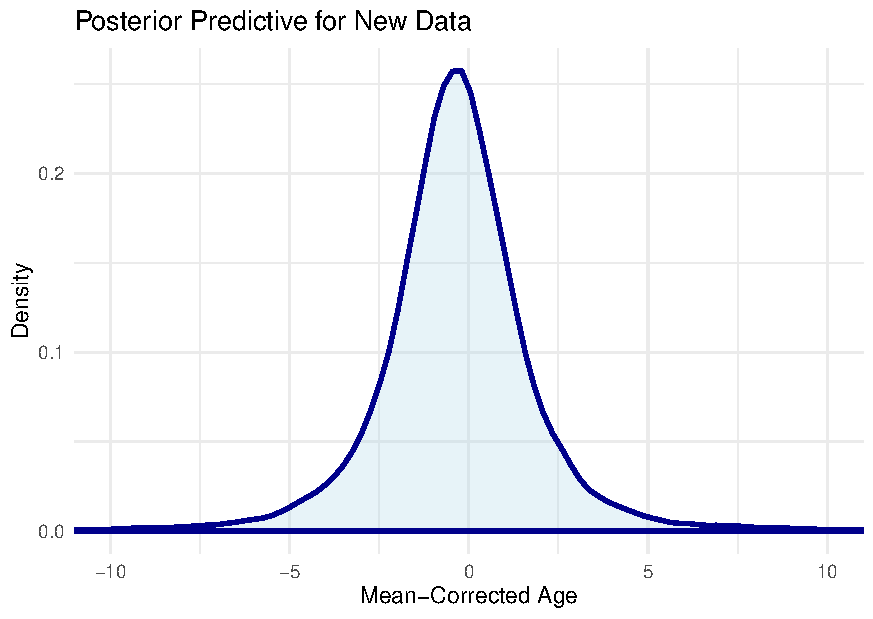
\includegraphics[width = 0.5\textwidth]{../pprednd}
	\caption{Posterior predictive density for new data}
	\label{fig:ppnd}
\end{figure}
\end{document}

